% lint-skip: 未完成ステータス（figure/table caption 未対応，人手チェック時に解消予定）
\documentclass[../../main.tex]{subfiles}
\begin{document}

\begin{flushright}
  \footnotesize\textit{【自動文字起こし・要確認】}
\end{flushright}

{\bf [解答]} 題意から
$$AQ : QB = PA : PB \cdots \text{①}$$
である．
\begin{figure}[H]
  \centering
  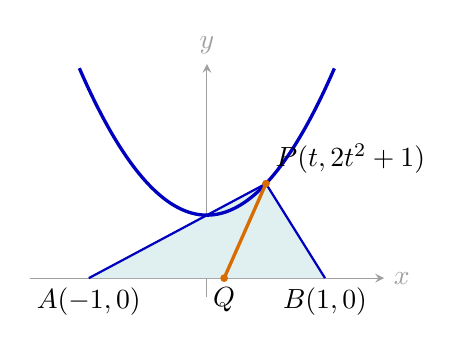
\begin{tikzpicture}[x=1.5cm,y=0.8cm,>=stealth]
    \coordinate (A) at (-1,0);
    \coordinate (B) at (1,0);
    % t=1/2 の例。角の二等分線から Q=(0.1459...,0)。
    \coordinate (P) at (0.5,1.5);
    \coordinate (Q) at (0.1459,0);
    \draw[->,gray!75] (-1.5,0)--(1.5,0) node[right] {$x$};
    \draw[->,gray!75] (0,-0.3)--(0,3.4) node[above] {$y$};
    \fill[teal!12] (A)--(P)--(B)--cycle;
    \draw[blue!75!black,very thick,domain=-1.08:1.08,samples=90]
    plot (\x,{2*\x*\x+1});
    \draw[blue!75!black,thick] (A)--(P)--(B);
    \draw[orange!85!black,very thick] (P)--(Q);
    \fill[orange!85!black] (P) circle (1.4pt) (Q) circle (1.4pt);
    \node[below] at (A) {$A(-1,0)$};
    \node[below] at (B) {$B(1,0)$};
    \node[below] at (Q) {$Q$};
    \node[above right] at (P) {$P(t,2t^2+1)$};
  \end{tikzpicture}
  \caption{放物線上の点 $P$ と，$AB$ 上の角の二等分線の交点 $Q$（図は $t=1/2$）}
\end{figure}

$$|AP|^2 = (t+1)^2 + (2t^2+1)^2$$
$$|PB|^2 = (t-1)^2 + (2t^2+1)^2$$
より，①から
$$\left(\dfrac{QB}{AQ}\right)^2 = \dfrac{|PB|^2}{|AP|^2} = \dfrac{(t-1)^2 + (2t^2+1)^2}{(t+1)^2 + (2t^2+1)^2} = f(t)$$
$\dfrac{QB}{AQ} > 0$ から，$f(t)$が最大，最小値をとる時，$\dfrac{QB}{AQ}$も最大，最小値をとる．

$f'(t)$の符号は，以下の式と同じ
\begin{align}
  g(t) &= \{2(t-1) + 2(2t^2+1) \cdot 4t\}\{(t+1)^2 + (2t^2+1)^2\} \\
  &\quad - \{2(t+1) + 2(2t^2+1) \cdot 4t\}\{(t-1)^2 + (2t^2+1)^2\} \\
  &= -4(2t^2+1)^2 + 8t(2t^2+1) \cdot 4t + 2(t-1)(t+1)^2 - 2(t+1)(t-1)^2 \\
  &= -4(2t^2+1) [ (2t^2+1) - 8t^2 ] + 2(t-1)(t+1) \cdot 2 \\
  &= 4( 12t^4 + 5t^2 - 2 ) = 4(3t^2+2)(4t^2-1)
\end{align}
従って，下表をえる

\begin{center}
  \begin{table}[htb]
    \centering
    \begin{tabular}{|c|c|c|c|c|c|}
      \hline
      $t$ & $\cdots$ & $-\dfrac{1}{2}$ & $\cdots$ & $\dfrac{1}{2}$ & $\cdots$ \\
      \hline
      $f'$ & $+$ & $0$ & $-$ & $0$ & $+$ \\
      \hline
      $f$ & $\nearrow$ & $\dfrac{9}{5}$ & $\searrow$ & $\dfrac{5}{9}$ & $\nearrow$ \\
      \hline
    \end{tabular}
  \end{table}
\end{center}

これと $f(t) = \dfrac{\left(2 + \dfrac{1}{t^2}\right)^2 + \dfrac{1}{t^2} \left(1 - \dfrac{1}{t}\right)^2}{\left(2 + \dfrac{1}{t^2}\right)^2 + \dfrac{1}{t^2} \left(1 + \dfrac{1}{t}\right)^2} \to 1 \ (t \to \pm\infty)$ から

$$\max \dfrac{QB}{AQ} = \sqrt{\dfrac{9}{5}} = \dfrac{3\sqrt{5}}{5}$$
$$\min \dfrac{QB}{AQ} = \sqrt{\dfrac{5}{9}} = \dfrac{\sqrt{5}}{3}$$

\end{document}
